% !TEX program = xelatex
%Wzór dokumentu
%tu zmień marginesy i rozmiar czcionki
    \documentclass[a4paper,12pt]{article}
	\usepackage{inputenc}[utf8]
    \usepackage[margin=2.5cm]{geometry}
    
 %Lepiej tego nie zmieniaj, jak co to dodawaj pakiety
	\usepackage{titlesec}
	\usepackage{titling}
	\usepackage{fancyhdr}
	\usepackage{mdframed}
	\usepackage{graphicx}
	\usepackage{amsmath}
	\usepackage{amsfonts}
	\usepackage{multicol}
	\usepackage{hyperref}
	\usepackage{float}
	\hypersetup{
		colorlinks=false,
		linkcolor=blue,
		filecolor=magenta,      
		urlcolor=cyan,
	}
	\usepackage{tikz}
	\usetikzlibrary{arrows}
	
%inny wygląd
	%\usepackage{tgbonum}
	
	
	%Zmienne, zmień je!
	\graphicspath{ {./ilustracje/} }
    \title{Ćwiczenia z Ekonomii}
    \author{Grzegorz Koperwas}
    \date{\today}
    
  %lokalizacja polska (odkomentuj jak piszesz po polsku)
  
    \usepackage{polski}
    \usepackage[polish]{babel} 
    \usepackage{indentfirst}
	\usepackage{icomma} 
	
    \brokenpenalty=1000
    \clubpenalty=1000
    \widowpenalty=1000    
 
 %nie odkometowuj wszystkiego, użyj mózgu
    %\renewcommand\thechapter{\arabic{chapter}.}
	\renewcommand\thesection{\arabic{section}.}
	\renewcommand\thesubsection{\arabic{section}.\arabic{subsection}.}
	\renewcommand\thesubsubsection{\arabic{subsubsection}.}

%Makra
    
\newcommand{\obrazek}[2]{
	\begin{figure}[h]
		\centering
		\includegraphics[scale=#1]{#2}
	\end{figure}
}     
            
    
    \newcommand{\twierdzonko}[1]{
        \begin{center}
        \begin{mdframed}
        #1
        \end{mdframed}          
        \end{center}
    } 
    
    \newcommand{\dwanajeden}[2]{
	\ensuremath \left( \begin{array}{c}
		#1\\
		#2
	\end{array} \right)
}  

\newcommand{\popytLewo}{\\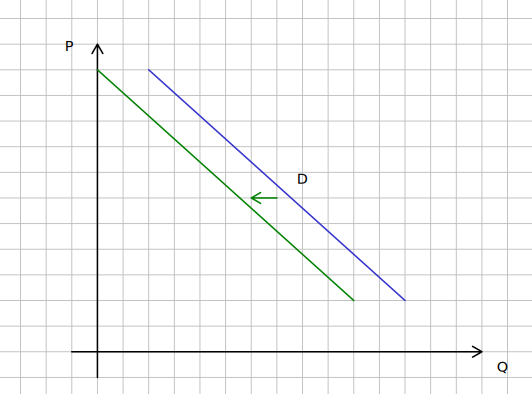
\includegraphics[scale=.33]{popytLewo.png}}
\newcommand{\popytPrawo}{\\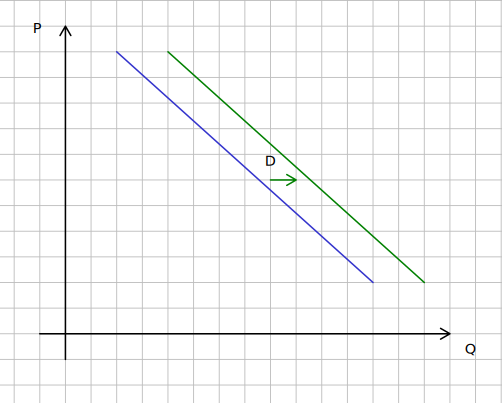
\includegraphics[scale=.33]{popytPrawo.png}}
\let\oldsection\section
\renewcommand\section{\clearpage\oldsection}

\titleformat{\section}
			{\bfseries\Large}
			{\thesection}
			{0.9ex}
			{}
			[\titlerule\vspace{1cm}]

\titleformat{\subsection}{\bfseries}{\large{Zad. \thesubsection}}{0.9ex}{}[\vspace{5mm}]

%Stopka i head (sekcja której nie powinno się zmieniać)
    \pagestyle{fancy}
    \fancyhead{}
    \fancyfoot{}
    
    %Zmieniaj od tego miejsca
	\rfoot{\thepage}
	\lfoot{Grzegorz Koperwas}
	\lhead{Numer Ćwiczeń: \thesection}
	\rhead{Ostatnia edycja: \today}
	\renewcommand{\headrulewidth}{1pt}
	\renewcommand{\footrulewidth}{1pt}

    
\begin{document}

\begin{titlepage}
	\maketitle
	\begin{center}
		Wydział Matematyki Stosowanej, Informatyka, Grupa 2C
	\end{center}
	\thispagestyle{empty}
\end{titlepage}
\setcounter{tocdepth}{1}
\tableofcontents
\pagebreak
\section{Pierwsze ćwiczenia:}


\subsection{Dlaczego ekonomia należy do nauk społecznych?}

Ekonomia należy do nauk społecznych ponieważ bada dystrybucje dóbr i zasobów w
\emph{społeczeństwie}, co jest jednym z procesów zachodzących w społeczeństwie.

\subsection{Z jakim okresem historycznym wiąże się naukowy rozwój ekonomii? Dlaczego?}

Ekonomia wyodrębniła się jako nauka pod koniec 18 wieku, wraz z początkami rewolucji
przemysłowej oraz po publikacji książki \emph{“The Wealth of Nations” Adama Smitha},
która to przyjęła tezę iż bogactwo danego kraju nie wynika z pełności skarbca monarchy,
lecz z przychodu narodowego.

\subsection{Jakie impulsy spowodowały powstanie teorii ekonomicznych?}

Impulsem dla powstania Teorii Ekonomicznych była potrzeba opisania nowych procesów w rodzących się pod koniec 18 wieku systemach kapitalistycznych, które zastępowały agrarne systemy feudalne. Przed ich powstaniem uważało się iż ziemia była głównym źródłem potęgi ekonomicznej kraju, gdyż system feudalny skupiał się właśnie na produkcji żywności z tejże ziemi.

Kolejnym z impulsów było upowszechnienie się narzędzi matematycznych oraz wczesne katastrofy ekonomiczne takie jak upadek \emph{Kompanii Mórz Południowych}.

\subsection{Porównaj definicje ekonomii \emph{A. Marshalla} ze współczesną jej definicją. Co łączy te definicje, co zaś różni?}

Definicja \emph{A. Marshalla} skupia się na relacji między ludźmi a dystrybucją zasobów materialnych. Nowoczesna ekonomia jest definiowana jako nauka społeczna o produkcji, dystrybucji oraz konsumpcji dóbr. Definicje te łączy uznanie ekonomi jako nauki badającej społeczeństwo jak i jego interakcje z dobrami, jednak \emph{definicja Marshalla} skupia się bardziej na badaniach społecznych, gdzie nowoczesna definicja skupia się bardziej na badaniu obiegu dóbr.

\subsection{Które [z] poniższych zagadnień mają charakter mikroekonomiczny, które zaś makroekonomiczny:}

\begin{enumerate}
	\item ,,Dlaczego obniżyła się cena jabłek?''

	      mikroekonomiczny

	\item ,,Dlaczego wzrósł poziom cen w Polsce,''

	      makroekonomiczny

	\item ,,Dlaczego wzrosło bezrobocie w Zabrzu''

	      mikroekonomiczny

	\item ,,Dlaczego wzrosło bezrobocie w Polsce''

	      makroekonomiczny

	\item ,,Dlaczego zmniejszyły się zyski w przemyśle tytoniowym''

	      mikroekonomiczny
\end{enumerate}

\subsection{Podaj inne przykłady problemów mikroekonomicznych i makroekonomicznych? (po 5 przykładów)}

\subsubsection*{Makroekonomiczne:}
\begin{itemize}
	\item Dlaczego zarobki Amerykańskiej klasy średniej spadają;
	\item Dlaczego wzrosła produktywność społeczeństwa;
	\item Jakie będą skutki załamania giełdy amerykańskiej;
	\item Obniżenie stóp procentowych;
	\item Spadek wzrostu PKB
\end{itemize}
\subsubsection*{Mikroekonomiczne:}

\begin{itemize}
	\item Spadek zarobków jednej rodziny.
	\item Załamanie się cen najmu przestrzeni sklepowej w Nowym Yorku.
	\item Drastyczne zwiększenie się cen nowych kart graficznych jednej firmy na wskutek ogromnego zapotrzebowania.
	\item Kolejne rewizje podręcznika wpływające negatywnie na rynek wtórny.
	\item Wygranie przetargu przez jedną firmę.
\end{itemize}

\subsection{Które z poniższych zdań są zdaniami ekonomii pozytywnej, które zaś ekonomii normatywnej:}

\begin{itemize}
	\item ,,ceny zabawek dla dzieci są za wysokie''

	      Ekonomia normatywna.

	\item ,,wzrost ceny jabłek powoduje zmniejszenie ilości nabywanych jabłek''

	      Ekonomia pozytywna.

	\item ,,Nakłady na badania naukowe są zbyt małe''

	      Ekonomia normatywna.

	\item ,,Wymiar podatku od dochodów osobistych w Polsce osłabia zainteresowanie staraniami o wzrost dochodów''?

	      Ekonomia pozytywna.
\end{itemize}

\subsection{Ustal, jaki charakter mają podane wypowiedzi - normatywny czy pozytywny:}

\begin{enumerate}
	\item ,,Popieram podniesienie płacy minimalnej, ponieważ pomoże to pracownikom niewykfalikowanym''

	      Normatywny, ponieważ autor wypowiedzi wyraża swoją subiektywną, ogólną opinię. Nie  uwzględnia on innych skutków \emph{podniesienia płacy minimalnej.}

	\item ,,Sprzeciwiam się podniesieniu płacy minimalnej, ponieważ spowoduje to wzrost bezrobocia w grupie młodych i niewykfalikowanych robotników''

	      Normatywny, ponieważ autor wyraża swoją subiektywną opinię, jednak popiera ją faktami z ekonomii pozytywnej.
\end{enumerate}

\subsection{Czy można uniknąć sądów oceniających zjawiska i procesy gospodarcze?}

Nie można uniknąć sądów nad zjawiskami i procesami ekonomicznymi, ponieważ ekonomia jako nauka społeczna, bada społeczeństwo. Jako iż te zjawiska są częścią procesów zachodzących w społeczeństwie, naturalne jest to iż społeczeństwo będzie miało swoje zdanie na ich temat, zatem będzie oceniać je według swoich subiektywnych opinii.

\subsection{Jak powinien być skonstruowany model domu studenckiego, jeżeli celem badawczym jest:}

\subsubsection*{Sposób powstawiania decyzji o wysokości miesięcznej opłaty za miejsce:}

Model \emph{sposobu powstawania decyzji o wysokości miesięcznej opłaty za miejsce} w domu studenckim składa się z:

\begin{itemize}
	\item Kosztów stałych utrzymania domu studenckiego.
	\item Regulacji prawnych regulujących opłaty oraz ulgi.
	\item Zapotrzebowania na miejsca.
	\item Stan domu studenckiego, lub/i kwota potrzebna na jego poprawę.
\end{itemize}

\twierdzonko{\paragraph{Odpowiedź:}
	Model składa się z zarządu podejmującego decyzję o wysokości opłaty.

	\vspace{0.6cm}
}

\subsubsection*{Opisanie sposobu rozwiązywania konfliktów między mieszkańcami:}

Model \emph{sposobu rozwiązywania konfliktów między mieszkańcami} w domu studenckim składa się z mieszkańców próbujących rozwiązywać swoje konflikty według regulaminu.

\subsection{Wróć do pytania 7 i odpowiedz, czy zdania, które uznałeś za zdania ekonomii pozytywnej, można bez zastrzeżeń uznać za twierdzenia naukowe?}

Zdania, które uznałam za zdania ekonomi pozytywnej można bez problemu uznać za twierdzenia naukowe, gdyż są tezami sugerującymi związek między zjawiskami które można mierzyć.

\subsection{Porównaj następujące zdania i wskaż, które jest poprawne pod względem naukowym:}


\begin{enumerate}
	\item ,,jeżeli rolnicy wydajnie pracują i jest urodzaj, to ogólny dochód rolników się zmniejszy''

	\item ,,jeżeli rolnicy wydajnie pracują i jest urodzaj, to ogólny dochód rolników prawdopodobnie się zmniejszy''
\end{enumerate}

Zdanie drugie jest poprawne pod względem naukowym gdyż stawia hipotezę. Zdanie pierwsze sugeruje istnienie powiązania nie dając na nie dowodów.

\subsection{Wyjaśnij paradoks zawarty w zdaniach z pytania 12 i ustal, która z zasadzek myślenia ekonomicznego została ominięta.}

W zdaniach z pytania 12 został zawarty paradoks w którym mimo iż rolnicy mają bardziej sprzyjające warunki, to ich dochody nie urosną. Jest to spowodowane tym że w czasach nieurodzaju plony rolne są towarami deficytowymi, bardziej rzadkimi, a zapotrzebowanie na nie pozostaje niezmienione.

Została ominięta zasadzka o tym iż zwiększona podaż wpłynie na popyt.

\subsection{Załóżmy, że celem działalności gospodarczej jest polepszenie jakości życia. Jak można mierzyć stopień realizacji tego celu?}

Mierzeniem jakości życia zajmuje się na przykład indeks ,,HDI\footnote{Human Development Index}'' w którym oprócz prognozowanej długości życia oraz dostępu do edukacji uwzględnia się dochody netto populacji oraz jej siłę nabywczą.

\subsection{,,Teoria musi opisywać rzeczywistość''. Zajmij stanowisko wobec tego zdania i uzasadnij je.}

Ekonomia, jako nauka społeczna, podlega pewnym rygorom metody naukowej. Z tego powodu poważne teorie powinny być oparte na obserwacjach, tutaj społeczeństwa. Z takiego rozumowania możemy łatwo dojść do konkluzji iż \emph{Teoria musi opisywać rzeczywistość}.

\subsection{Ustal, które z następujących zdań jest hipotezą:}

\begin{itemize}
	\item ,,koty widzą w ciemności lepiej niż psy''

	      Nie jest to hipoteza

	\item ,,ludzie, którzy się częściej opalają, są bardziej narażeni na chorobę nowotworową skóry''

	      Nie jest to hipoteza

	\item ,,jeżeli dochody rosną, to ludzie konsumują więcej dóbr''

	      Jest to hipoteza

	\item ,,jeżeli ludzie uwierzą, że dany produkt jest szkodliwy dla zdrowia, to będą go mniej konsumować''

	      Jest to hipoteza
\end{itemize}

\subsection{Czy przy formułowaniu hipotez musi być stosowana zasada ceteris paribus?}

Zasada \emph{Ceteris paribus} musi być stosowana przy formułowaniu hipotez po to by oddzielić zmienne które mogą wpływać na wynik, od zmiennych które dana hipoteza opisuje.

\subsection{Dlaczego modele ekonomiczne należy traktować poważnie, lecz nie dosłownie?}

Modele ekonomiczne są uproszczeniem procesów zachodzących w gospodarce, a nie jej dokładną symulacją. Z tego powodu powiliśmy brać wyniki analiz za pomocą ich przeprowadzonych pod uwagę, lecz musimy pamiętać iż nikt nie jest w stanie w pełni przewidzieć przyszłości.

\subsection{Czy politycy mogą ignorować teorie ekonomiczne?}

Politycy mogą ignorować teorie ekonomiczne jednak muszą pamiętać o konsekwencjach swoich wyborów. Tak jak ja mogę nie zrobić zadań z \emph{podstaw ekonomii}, tak polityk może zacząć ignorować teorie ekonomiczne, lub powoływać się na nieprawdziwe teorie\footnote{Na przykład \emph{trickle down economics}}, jednak musi on pamiętać że z jego wyborów rozliczą go wyborcy lub inne wpływowe osoby.

\subsection{,,Teorie raz uznane za prawdziwe są zawsze uznawane za prawdziwe''. Czy zgadzasz się z tym stwierdzeniem.}

Tak jak zmienienie swojej opinii na dany temat nie jest niczym złym, tak zmienienie opinii na temat danej teorii przez środowisko naukowe nie jest niczym nadzwyczajnym.

Wiele teorii było kiedyś uznawanych za prawdziwe, czy mówimy tu o \emph{płaskiej ziemi}, o tym czy \emph{rząd nie powinien się w jakimkolwiek stopniu angażować w gospodarkę} czy \emph{merkantyliźmie}, jednak obecnie uznaje się je za obalone.

\section{Ćwiczenia drugie - 26.10.2020}

\subsection{Ustal, jakie rzeczy, usługi lub stany służą bezpośrednio do zaspokajania potrzeb:}

\begin{itemize}
	\item biologicznych - jedzenie
	\item bezpieczeństwa - zamki do drzwi
	\item kontaktów społecznych - usługi typu komunikatory internetowe
	\item uznania - media społecznościowe
	\item samorealizacji - książki
\end{itemize}

\subsection{Podaj po kilka przykładów dóbr ekonomicznych i dóbr wolnych:}

\subsubsection*{Dobra ekonomiczne:}

\begin{itemize}
	\item Telefony
	\item Oprogramowanie
	\item Urządzenia elektroniczne
	\item Muzyka
\end{itemize}

\subsubsection*{Dobra wolne}

\begin{itemize}
	\item Gleba
	\item Woda
	\item Minerały
	\item Pasma radiowe
\end{itemize}

\subsection{Co stanowi kryterium podziału dóbr na konsumpcyjne i produkcyjne?}

Dobra konsumpcyjne są konsumowane przez finałowego konsumenta. Nie są wtedy używane do tworzenia dalszych dóbr.

Dobra produkcyjne są używane do produkcji innych dóbr.

\subsection{Czy to samo dobro może być dobrem konsumpcyjnym i dobrem produkcyjnym?}

Tak, jednym z takich dóbr jest chleb, który jest dobrem konsumpcyjnym, oraz jest również używany do produkcji kanapek.

\subsection{Czy dobro inwestycyjne jest tym samym co dobro kapitałowe?}

Dobra inwestycyjne to to samo co dobra kapitałowe.

\subsection{Kwadracik:}

\obrazek{0.5}{kwadrat.png}

\subsection{,,W krajach Europy Zachodniej masło nie jest dobrem rzadkim''. Zajmij stanowisko wobec tego stwierdzenia i uzasadnij je.}

Masło nie jest dobrem rzadkim ponieważ jest jego produkowana ograniczona ilość, która jest na tyle mała iż zachodzi import masła\footnote{\url{https://foodfakty.pl/eksport-serow-i-masla-z-polski-wiekszy-niz-przed-rokiem}} z innych krajów Unii Europejskiej. Jest to spowodowane ograniczoną produkcją mleka tłustego, z którego są produkowane śmietany itp.

Jednak warto zauważyć iż mleko odtłuszczone, te które kupujemy w sklepach, staje się praktycznie dobrem rzadkim. Jest one praktycznie \emph{odpadem} przy produkcji innych produktów mlecznych i często dochodzi do sytuacji gdzie jest one tańsze od wody lub bardziej opłaca się je wylewać niż sprzedawać.\footnote{\url{https://time.com/4530659/farmers-dump-milk-glut-surplus/}}

\subsection{Przypomnij sobie definicję ekonomii. Dlaczego ekonomia zajmuje się dobrami rzadkimi? W jakim aspekcie zajmuje się również dobrami wolnymi?}

Ekonomia zajmuje się dobrami rzadkimi, ponieważ to jak ludzie, jako istoty społeczne, zarządzają ograniczoną ilością zasobów jest ciekawe oraz zrozumienie tych procesów pozwala nam na próby ich poprawy. Systemy ekonomiczne i ich metody dystrybucji dóbr rzadkich definiują instytucje państwowe. Wadliwe systemy ekonomiczne takie jak hiszpańska \emph{,,Encomienda''} pozostawiają swoje ślady w społeczeństwach ameryki łacińskiej do dziś.\footnote{Polecam wideo-lekturę filmu o skutkach \emph{Encomiendy} w Meksyku \url{https://youtu.be/SPs6tjXsf7M} [ENG]}

Dobra wolne, mimo iż z definicji nie są ograniczone, również posiadają swoje procesy dystrybucji, które mogą być przedmiotem rozważań nauki społecznej jaką jest ekonomia.

\subsection{,,Piasek pustynny zawsze będzie dobrem wolnym, ponieważ jego ilość przekracza potrzeby ludzkie''. Czy zgadzasz się z tym stwierdzeniem?}

Piasek pustynny może nie jest materiałem tak rzadkim jak piasek plażowy, który bywa nawet kradziony\footnote{\tiny{\url{https://www.theguardian.com/global/2018/jul/01/riddle-of-the-sands-the-truth-behind-stolen-beaches-and-dredged-islands}}}, jednak kto wie, może kiedyś zapotrzebowanie na piasek pustynny wzrośnie wobec rosnących kosztów piasku plażowego oraz opracowania jakiejś metody przetwarzania ziaren na inne rozmiary.

Nigdy nic nie wiadomo, jednak kopanie piasku na środku pustyni nie jest tak prostą sprawą, głównie z powodu obecnie istniejącej infrastruktury lub jej braku. Z tych powodów piasek pustynny może się łatwo stać dobrem rzadkim, z powodu trudności w eksploatacji.

\subsection{Ziemia ta była dobrem wolnym czy rzadkim?}

Rzadkim, iż jej ilość była skończona.

\subsection{Ustal listę poszczególnych czynników produkcji niezbędnych do eksploatacji złóż ropy naftowej:}
\begin{itemize}
	\item Wiedza na temat sposobów wydobycia ropy.
	\item Pracownicy
	\item Odpowiednie maszyny i narzędzia.
	\item Pojazdy lub rurociąg do przewozu ropy.
	\item Urządzenia bezpieczeństwa wymagane prawnie.
\end{itemize}

\subsection{Co poza ilością poszczególnych czynników produkcji decyduje o wyniku produkcyjnym?}

\begin{itemize}
	\item Regulacje prawne.
	\item Zdarzenia losowe.
\end{itemize}

\subsection{Ustal, które z tych wielkości są zasobami, a które strumieniami?}

\begin{itemize}
	\item konsumpcja - strumień
	\item inwestycja - zasób
	\item dług - zasób
	\item koszt - zasób
	\item płaca - strumień
	\item podatek - strumień / zasób
	\item majątek - zasób
	\item dochód - strumień
\end{itemize}

\subsection{Zinterpretuj czynniki produkcji:}

Strumienie:
\begin{itemize}
	\item praca
\end{itemize}
Zasoby:
\begin{itemize}
	\item ziemia
	\item kapitał
\end{itemize}

\subsection{Jak są mierzone zasoby i strumienie:}
\begin{enumerate}
	\item na koncie bankowym
	      \begin{itemize}
		      \item strumień - zmiana w czasie
		      \item zasób - stan konta
	      \end{itemize}
	\item za pomocą gazomierza
	      \begin{itemize}
		      \item strumień - zmiana wskazania od ostatniej kontroli
		      \item zasób - stan licznika
	      \end{itemize}
\end{enumerate}

\subsection{Czy dobra wolne są przedmiotem podziału.}

Nie, gdyż ich ilość jest bliska nieskończoności.

\subsection{Czy podział dóbr rzadkich za pośrednictwem rynku eliminuje ich rzadkość?}

Nie, ponieważ rynek nie gwarantuje podziału dóbr w taki sposób by zadowolić potrzeby każdej jednostki.

\subsection{Czy może się zdążyć naruszenie suwerenności konsumenta?}

Tak jeżeli:

\begin{itemize}
	\item Na rynku panuje monopol narzucający konsumentowi dany wybór.
	\item Koszt zmiany wybranego producenta jest zbyt wysoki z powodu niestandaryzowanych rozwiązań.

	      Przykładem jest firma \emph{Apple} gdzie konsument korzystający z jej rozwiązań nie może łatwo integrować produktów konkurencji, tylko musi płacić więcej za rozwiązanie firmy \emph{Apple}. Na przykład do aktualizacji firmware na słuchawkach bezprzewodowych jest potrzebny telefon marki \emph{iPhone} itd.
\end{itemize}

\subsection{,,W gospodarstwie domowym odbywa się konsumpcja, w przedsiębiorstwie zaś odbywa się produkcja''}

Przedsiębiorstwa również konsumują dobra czy to w celu wyprodukowania innych dóbr, zarządzania sobą czy po prostu są konsumowane w celach wizerunkowych czy innych nie związanych bezpośrednio z produkcją.
Jeżeli dane gospodarstwo domowe zajmuje się produkcją jakiegoś dobra, to staje się częściowo przedsiębiorstwem.

\section{Metody dokonywania wyborów ekonomicznych}

\subsection{Podaj przykłady społeczności prowadzących w przeszłości lub obecnie:}

\begin{enumerate}
	\item Działalność tradycyjną - Społeczeństwa epoki kamienia.
	\item Działalność nakazową - Społeczeństwo starożytnego egiptu w epoce brązu z centralnym planowaniem gospodarki rolnej.
	\item działalność w gospodarce rynkowej - Obecne społeczeństwo polskie.
\end{enumerate}

\subsection{Czy w gospodarce zwyczajowej mogą być racjonalne wybory ekonomiczne, działalność ekonomiczna?}
W gospodarce zwyczajowej racjonalność wyborów ekonomicznych jest ograniczona, gdyż podlegają one zmianie wówczas kiedy stają się one niemożliwe, na przykład z powodu ostrej zmiany cen na rynku. Zatem w gospodarce zwyczajowej mogą istnieć racjonalne wybory ekonomiczne i działalności, jednak z biegiem czasu dochodzi do erozji racjonalności wyborów aż do osiągnięcia pewnego punktu wymuszającego zmianę wyboru.

\subsection{Firma działająca w gospodarce rynkowej ogłosiła upadłość. Zinterpretuj ten fakt pod kątem racjonalności gospodarczej.}

Jeśli firma w gospodarce rynkowej ogłosiła upadłość to wskazuje to na brak istnienia racjonalnych powodów dla jej dalszego funkcjonowania.

\subsection{,,Racjonalnie działająca jednostka w swoich wyborach nie ulega emocjom, nie kieruje się tradycją'' - Zajmij stanowisko}

Racjonalna jednostka \emph{Homo economicus} powinna zawsze w pełni racjoalnie bez zważania na inne czynniki subiektywne dokonywać wyborów, jednak w praktyce takie jednostki nie istnieją. Jednostka nie może posiadać wszystkich informacji potrzebnych do w pełni racjonalnego wyboru, zatem uzupełnia je sobie swoimi emocjami i doświadczeniami wynikającymi z tradycji, na przykład ,,Mój poprzedni telefon by od LG, zatem sobie kupię nowy model tej samej marki bo mi się podobał''.

\subsection{Wskaż, jak każda z następujących zmian może wpływać na twoje decyzje o podjęciu opisanych zadań.}

\begin{itemize}
	\item Spadek temperatury powietrza z 25 stopni celsjusza do 20 stopni na decyzję o pływaniu - wybiorę pływalnie krytą zamiast kąpieliska.
	\item Zmiana czasu rozpoczynania wykładu z 11:00 na 8:00 na decyzję o pójściu na wykład - Jeśli wykład jest nudny to nie pójdę na wykład.
	\item Wzrost ceny wieprzowiny na decyzję o jedzeniu kotletów - Chętniej będę jadł swoje kotlety drobiowe.
	\item Wzrost czynszu mieszkaniowego na decyzję o budowie domu - Zacznę analizować swoje perspektywy kredytowe.
\end{itemize}

\subsection{,,Zasada racjonalnego gospodarowania głosi, że należy użyć najmniej środków, aby osiągnąć cel w najwyższym stopniu'' - Zajmij stanowisko}

Jeśli w celu osiągnięciu danego celu będziemy marnować zasoby poprzez nie używanie najmniejszej możliwej ich ilości to sugeruje to możliwość lepszego osiągnięcia celu. Jednakże należy pamiętać żeby stwierdzić że, dane zasoby są marnowane należy dobrze rozpoznać cel. Przykładowo cel zawierający w sobie zmotywowaną załogę fabryki nie marnuje zasobów poprzez wyższe wypłaty.

\subsection{,,Homo oeconomicus to niemoralne, egoistyczne indywiduum'' - Zajmij stanowisko}

\emph{Homo oeconomicus} jako idealnie racjonalna jednostka mająca jeden jedyny cel zaspokojenia swoich potrzeb jest z definicji osobą egoistyczną, nie zależy mu na zaspokojeniu potrzeb innych. Mam nadzieje iż możemy się zgodzić iż osoba nie przejmująca się jakkolwiek losem innych osób nie jest osobą moralną, gdyż nie przejmuje się ona jakimkolwiek wyzyskiem innych osób poza nią.

\subsection{Omów ograniczenia, które wywierają wpływ na decyzje:}

\begin{itemize}
	\item najbiedniejszej osoby na świecie - Posiadany kapitał (lub jego brak)
	\item najbogatszej osoby na świecie - Moralność
	\item firmy w Szwajcarii - Koszt łamania regulacji prawnych
	\item agencji rządowej w Chinach - Struktury władzy w Komunistycznej Partii Chin
	\item ludności świata - wielkości posiadanego kapitału, prawa fizyki.
\end{itemize}

\subsection{Jeśli będziesz rektorem Politechniki, to co zrobisz, gdy budżet uczelni zostanie zmniejszony o 5\%, 20\% i 50\%}

\begin{enumerate}
	\item 5\% - Szukanie możliwości zdobycia funduszy w inny sposób, zwiększenie ilości studentów w grupach na pierwszym roku.
	\item 20\% - Patrz punkt poprzedni $+$ Zaprzestanie dotowania organizacji nie przynoszących dochodów bezpośrednio
	\item 50\% - Patrz punkt poprzedni $+$ Zatrzymanie inwestycji w infrastrukturę, sprzedaż nieruchomości,
\end{enumerate}

\subsection{Wynajmujesz mieszkanie, za które płacisz właścicielowi 20 tys. PLN rocznie. Twoje oszczędności w wysokości 200 tys. PLN są ulokowane na koncie ban­kowym na 15\% rocznie. Mieszkanie można nabyć za 200 tys. PLN.}

\emph{Czy zdecydujesz się na kupno mieszkania? Ustal korzyść i alternatywny koszt zakupu mieszkania.}


Decyduje się na zakup mieszkania gdyż jest ono dobrem które nie traci na obecnym rynku na wartości. To co zaoszczędzę na czynszu będę mógł ulokować na lokacie z powrotem. Na obecnym, rynku ceny mieszkań rosną więc jest to też swego rodzaju inwestycja.

\subsection{Mając do dyspozycji 100 tys. PLN stajesz przed wyborem jednej z poniższych możliwości}

\begin{itemize}
	\item lokata na koncie bankowym o rocznym oprocentowaniu wynoszącym 30\%
	\item kupno obligacji Skarbu Państwa, które przynoszą 35 tys. PLN rocznego dochodu
	\item kupno akcji spółek notowanych na giełdzie, od których dywidenda wyniesie średnio 20\% rocznie.
\end{itemize}

Większość pieniędzy inwestuje w obligację Skarbu Państwa, część inwestuje w giełdę by mieć możliwość szybkiej ich wypłaty.

\subsection{Prowadzisz sklep z owocami i warzywami. Codziennie pozostają ci kartonowe opakowania. Koszt załadowania i przewiezienia opakowań do firmy zajmującej się ich skupem wynosi 2 PLN za 1 kg. }

\emph{Jaką podejmiesz decyzję, gdy cena opa­kowań wynosi:}

\begin{itemize}
	\item 1,5 zł
	\item 2 zł
	\item 2,5 zł za kg
\end{itemize}

Jeśli koszt przechowywania kartonów jest nie zerowy (na jednostkę czasu) będę się starał przewozić zawszę do firmy je skupującej. W innym przypadku będe je przewozić jeśli cena skupu jest większa niż 2 zł.

\subsection{Ulokowałeś 100 tys. PLN w akcjach spółek notowanych na giełdzie, przy­noszących 20\% rocznej dywidendy. W wyniku hossy zarobiłeś dodatkowo 5 tys. PLN, które możesz przeznaczyć na sfinansowanie wakacji lub na nabycie dodatkowych akcji.}

\emph{Ceny wycieczek zagranicznych wzrosną w ciągu roku prawdopodobnie o 30\%.
	Na co przeznaczysz 5 tys. PLN? Uzasadnij odpo­wiedź.}

\vspace{1cm}

Zarobione 5000 zł przeznaczę na wycieczkę zagraniczną, ponieważ zysku z giełdy z kwoty 5000 zł będą mniejsze od wzrostu cen wycieczek zagranicznych.

\section{Rynek i Gospodarka Rynkowa}

\subsection{Posiadasz biżuterię, która przestała ci się podobać, a chcesz mieć samochód.}

\emph{Porównaj swój sposób postępowania w:}

\begin{itemize}
	\item w warunakch wymiany barterowej - Znalezienie osoby która:
	      \begin{itemize}
		      \item Posiada samochód
		      \item Podoba się jej moja biżuteria
	      \end{itemize}
	      lub zacznę poszukiwania trzeciego dobra i osoby trzeciej która za biżuterię odda mi dobro za którę nabędę samochód.
	\item Towarowo - pieniężnej - Uniwersalne dobro to pieniądz - sprzedam więc osobie trzeciej biżuterię, a za otrzymane pieniądze kupię samochód.
\end{itemize}

\subsection{Załóżmy, że w 1989r. dobro X kosztowało 100 PLN, a w 1993r. jego cena była równa 700 PLN.}

\emph{Gdy cena innych dóbr w 1993 wzrosły w porównaniu z 1989 o 100\%, cena relatywna dobra X wzrosła czy zmalała?}

\begin{align*}
	100 \cdot \left(1 + 100 \%\right) = 100 \cdot 2 & = 200                                           \\
	200                                             & < 700 \Rightarrow \text{Cena relatywna wzrosła}
\end{align*}

\subsection{Wypełnij tabelę}

\emph{Nazwij ceny nakładu i zasobu odpowiedniego czynnika produkcji.}

\begin{table}[h]
	\begin{tabular}{|c|c|c|}
		\hline
		Wyszczególnienie  & \multicolumn{2}{c|}{Cena}                              \\
		                  & nakładu czynnika produkcji & zasobu czynnika produkcji \\\hline
		Ziemia            & koszt eksploatacji         & ilość ziemi               \\
		Praca             & płaca                      & -                         \\
		Kapitał rzeczowy  & maszyny                    & Wytworzenie Dobra         \\
		Kapitał pieniężny & oprocentowanie             & Wartość zysku             \\\hline
	\end{tabular}
	\centering
\end{table}

\subsection{Co to znaczy że rynek jest doskonale przejrzysty.}

Na rynku doskonale przejrzystym każda, z uczestniczących w rynku organizacji posiada dostęp do wszystkich możliwych informacji na rynku.

Na rynku nie doskonale przejrzystym jednostki w nim uczestniczące nie mają dostępu do wszystkich informacji na nim. Przykładowo statystyczny Polak nie zna cen na wszystkich stacjach benzynowych w Polsce.

\subsection{Na czym polega różnica między rynkiem wolnym a czarnym?}

Na rynku wolnym podmioty mogą zawierać transakcje bez nacisku ze strony podmiotów trzecich. Rynek czarny jest rynkiem który jest charakteryzowany przez nacisk ze strony państwa z powodu nielegalności przedmiotu transakcji, podmiotów zawierających transakcję czy okoliczności transakcji.

\subsection{Uzasadnij następujące stwierdzenie:}

\textbf{,,System cen jest systemem informacji dla podmiotów gospodarczych''}

\vspace{.3cm}

Cena ustalana przez sprzedawcę jest informacją dla kupujących jaką wartość (według sprzedawcy) posiada dane dobro. Podobna zachodzi sytuacja w drugą stronę, gdzie kupujący poprzez chęć kupna czy oferowaną cenę przekazują sprzedawcom informację o wartości dobra.

\subsection{W jakim sensie mechanizm rynkowy racjonuje rzadkie dobra i usługi?}

Mechanizm rynkowy racjonuje rzadkie dobra i usługi poprzez rozdanie ich osobą które najbardziej ich potrzebują, zatem przypisują im największą wartość. Ma to jednak wadę wynikającą z tego iż dla niektórych dóbr, których wartość dąży do nieskończoności\footnote{Na przykład rynek ludzkich organów i usług medycznych}, mechanizmy rynkowe przypisywałyby je tylko jednostką z największą ilością kapitału, a nie jednostką które potrzebują ich najbardziej.

\subsection{Wykaż, że wzrost ceny jest funkcją rzadkości dobra:}

Dla stałego zapotrzebowanie na dane dobro\footnote{na przykład ropę naftową}, w przypadku wzrostu produkcji (spadku rzadkości), producenci będą się starali pobudzić popyt poprzez obniżenie cen, gdyż każdy producent będzie chciał sprzedać swoją nadwyżkę. Jeśli jakiś producent nie obniży swojej ceny to nie sprzeda swoich dóbr, więc jest zmuszony do tejże obniżki cen, obniżki będą trwały aż pobyt wyrówna się z podażą dla nowej ceny produktu.

Jednakże z tych stwierdzeń wynika iż \emph{cena} jest funkcją rzadkości dobra, a nie jej wzrost, który jest pochodną (zmianą) funkcji rzadkości.

\subsection{Schemat okrężnego przepływu dóbr i usług konsumpcyjnych, czynników produkcji oraz pieniądza w gospodarce rynkowej}

\obrazek{0.5}{schemat1.png}

\section{Popyt i podaż}

\subsection{Zaprojektuj badanie popytu na rowery w Katowicach}

Badanie składało by się z analizy trendów na podstawie danych z przeszłości oraz danych obecnych:

\subsubsection*{Badania tendencji historycznych}

Zgromadzenie historycznych danych z lat ubiegłych takich jak:

\begin{itemize}
	\item Ilość sprzedawanych rowerów w danych półkach cenowych.
	\item Ceny sprzedawanych rowerów (z uwzględnieniem inflacji itp.)
	\item Popularność wszelakich usług wypożyczania rowerów.
	      Tutaj możliwa by była pewnie analiza demografii użytkowników tych usług.
\end{itemize}

Na ich podstawie można by było zobaczyć w jaką stronę przesuwają się trendy, a tym samym jak będzie się zmieniać popyt.

\subsubsection*{Analiza danych obecnych}

Zgromadzenie danych z obecnego roku takich jak:

\begin{itemize}
	\item Ilość sprzedanych rowerów wraz z ceną każdej sztuki, lub dane uśrednione. Idealnie wraz z danymi z portali aukcyjnych. Mile widziane byłyby również danie o majętności kupujących.
	\item Ilość użytkowników usług wypożyczania rowerów.
\end{itemize}

Dzięki tym danym można by było określić jaką część swoich pieniędzy są chętni wydać na rowery mieszkańcy Katowic.


\subsection{Jak często chodzisz do kina? Ile rzadziej chodziłbyś gdyby bilet byłby dwukrotnie droższy? Odróżnij swoją krzywą popytu na bilety kinowę i faktyczną liczbę biletów nabywanych przy bieżącej cenie}

Nawet w latach ubiegłych do kina chodziłem średnio rzadziej niż raz do roku. Podwyższenie cen biletów prawdopodobnie nie wpłynęłoby wogóle na mój popyt, gdyż procesie podejmowania moich decyzji dużo większe znaczenie ma film, na którego obejrzenie się mam udać.

Moja krzywa popytu, która właściwie jest prostą, jest raczej różna od ogólnej krzywej. Osoby, które często chodzą do kina będą bardziej zwracały uwagę na cenę biletu, osoby które chodzą do kina od święta, nadal będą chodzić do kina rzadko.

\subsection{Znajdź dwa błędy w następujących zdaniach:}

\paragraph*{,,Jeżeli cena wołowiny rośnie, to popyt na wołowinę się zmniejsza''} - Popyt jest funkcją, nie wartością. Dla danej ceny \emph{zwraca on nam} daną liczbę sztuk którą kupią konsumenci.

\paragraph*{,,Ekonomiści szacują, że wzrost ceny wołowiny o 5\% spowoduje spadek popytu o 1\%''} -  Popyt jest funkcją, nie wartością. Dla danej ceny \emph{zwraca on nam} daną liczbę sztuk którą kupią konsumenci.

\[
	\text{sztuki kupione} \cdot 0,99 = \text{funkcja popytu}\left(\text{cena} \cdot 1,05 \right)
\]

\subsection{Wskaż, które z następujących zdarzeń należy zilustrować za pomocą przesunięcia krzywej popytu, a które za pomocą ruchu wzdłuż krzywej}

\begin{enumerate}
	\item ,,ceny samochodów obniżyły się ceteris paribus'' Wzdłuż krzywej
	\item ,,wzrosła trzykrotnie cena benzyny ceteris paribus'' Przesunięcie krzywej
	\item ,,ceny biletów na komunikację zbiorową obniżyły się 10krotnie'' Przesunięcie krzywej
	\item ,,zmniejszyły się dochody społeczeństwa'' Przesunięcie krzywej
	\item ,,w związku z nałożeniem podatku akcyzowego na samochody oczekiwany jest wzrost cen samochodów ceteris paribus'' Wzdłuż krzywej
\end{enumerate}

\subsection{Wskaż, które z następujących zdarzeń należy zilustrować za pomocą przesunięcia krzywej popytu, a które za pomocą ruchu wzdłuż krzywej}

\begin{itemize}
	\item ,,Wzrost cen mleka ceteris paribus spowodował spadek konsumpcji mleka'' - ruch wzdłuż
	\item ,,Gdy wzrosły dochody konsumentów ceteris paribus, wzrosło kupno samochodów [sic]'' - Przesunięcie
\end{itemize}

\subsection{Pokaż jak przesunie się krzywa popytu}

\begin{itemize}
	\item Na rynku obuwia zimowego, gdy zwiększyły się opady śniegu ceteris paribus - W górę
	\item Na rynku herbaty, gdyby cena kawy wzrosła ceteris paribus - W górę
	\item Na rynku herbaty, gdyby wzrosła cena cukru - Brak ruchu
\end{itemize}

\subsection{Podaj cztery przykłady czynników, które mogą spowodować zmianę popytu na ryby.}

\begin{itemize}
	\item Skandal humanitarny na jednej z ferm rybnych / kutrów rybackich \popytLewo
	\item Tradycje, na przykład świąteczne. \popytPrawo
	\item Zmiany rzadkości ryb poprzez zbyt mocne przełowienie. \popytLewo
	\item zmniejszenie się powszechności tradycji takich jak jedzenie ryb w piątki \popytLewo
\end{itemize}

\subsection{Z prawa popytu wynika, że ceny się nigdy nie zmieniają! [...] Czy to stwierdzenie jest prawdziwe?}

Z prawa popytu wynika iż cena jest wypadkową popytu i podaży, zatem w idealnym przypadku się nie zmienia chyba że zmieni się popyt lub podaż.

\subsection{Jakie zmienne, oprócz ceny danego dobra, wywierają taki wpływ na nabywaną ilość tego dobra jak ona?}

\begin{itemize}
	\item Efekt owczego pędu - trendy
	\item Dochód populacji
	\item Spekulacje - jeśli przewidywany jest bliski wzrost ceny, popyt wzrośnie chwilowo.
\end{itemize}

\subsection{Narysuj prawdopodobne przesunięcie krzywych popytu na:}

\begin{itemize}
	\item Podróże koleją, gdyby skrócono czas przejazdu \popytPrawo
	\item Samochody, gdyby wzrosły ceny biletów kolejowych \popytPrawo
	\item Elektryczność, gdyby przeciętna temperatura powietrza w Polsce się podniosła ceteris paribus \popytPrawo
\end{itemize}

\subsection{Uzasadnij, które z następujących dóbr mogą mieć krzywą popytu o pozytywnym nachyleniu}

Diamenty posiadają pozytywną krzywą popytu, spowodowaną zabiegami marketingowymi które sprawiają iż są one postrzegane jako dobro bardzo rzadkie. W rzeczywistości są one dość powszechne oraz stosowane często do zastosowań przemysłowych. Diamenty przemysłowe z powodu swojej niskiej ceny nie są postrzegane jako dobro luksusowe, zatem popyt zwykłych konsumentów na nie jest stosunkowo niski.

\section{Powtórzenie wiadomości - mikroekonomia.}

\subsection{Dopasuj pojęcia do definicji:}

\subsubsection*{Makroekonomia}

Dział ekonomii zajmujący się badaniem gospodarki jako całości.

\subsubsection*{Mikroekonomia}

Dział ekonomii badający zachowania podmiotów gospodarujących, rynki na których podmioty te działają oraz powiązania występujące pomiędzy podmiotami i pomiędzy rynkami.

\subsubsection*{Sądy pozytywne w ekonomii}

Bezstronne ustalanie prawidłowości zachodzących w gospodarce na podstawie zaobserwowanych faktów.

\subsubsection*{Sądy normatywne w ekonomii}

Subiektywne, wartościujące opinie na temat gospodarki.

\subsubsection*{Czynniki produkcji}

W warunkach ograniczonych zasobów, chęć zwiększenia produkcji jednego dobra o kolejne jednostki będzie wymagała rezygnacji z coraz większej części produkcji drugiego dobra.

\subsubsection*{Polityka restrykcyjna}

Działania polegające na hamowaniu aktywności gospodarczej w warunkach bardzo dobrej koniunktury.

\subsubsection*{Zasoby}

Wielkości, których właścicielami są gospodarstwa domowe, a nabywane przez przedsiębiorstwa, umożliwiają produkcję.

\subsubsection*{Zmienne endogeniczne}

Zmienne, które nie są objaśniane, przyjmowane są jako dane.

\subsubsection*{Zmienne egzogeniczne}

Zmienne, które objaśniane są przy wykorzystaniu znajomości zasad panujących w gospodarce.

\subsubsection*{Krzywa możliwości produkcyjnych}

Pokazuje kombinację produkcji dwóch dóbr, przy założeniu, że czynniki produkcyjne są wykorzystane w pełni i w sposób efektywny

\subsubsection*{Koszt alternatywny}

W warunkach ograniczonych zasobów, koszt związany w niewykorzystaniem lub utratą najlepszej alternatywnej możliwości.

\subsubsection*{Prawo rosnących kosztów względnych}

\subsubsection*{Wartości nominalne}

Inaczej, wartości wyrażone w cenach stałych.

\subsubsection*{Wartości realne}

Inaczej, wartość wyrażona w cenach bieżących. Wpływ na jej kształtowanie się mają zmiany ilości i/lub zmiany cen.

\subsubsection*{Modelowanie makroekonomiczne}

Poszukiwanie matematycznych zależności za pomocą modeli ekonomicznych, pomiędzy zmiennymi makroekonomicznymi.

\subsection{Pytania problemowe:}

\subsubsection{Jaka jest zasadnicza różnica miedzy gospodarką naturalną a gospodarką rynkową?}

Zasadniczą różnicą jest występująca w gospodarce rynkowej specjalizacja siły roboczej, wymiana dóbr i brak jednostek które są w pełni samodzielne.

\subsubsection{Czym się różnią strumienie od zasobów?}

Zasób jest wartością nie zależną od czasu, strumień jest zmianą wartości zasobu w czasie, z zastrzeżeniem iż magazynowanie części strumieni, takich jak energia elektryczna jest drogie lub/i nie możliwe.

\subsubsection{Jak jest podstawowa różnica pomiędzy dobrami prywatnymi a dobrami publicznymi?}

Dobra prywatne są zarządzane przez jedną jednostkę - właściciela. Dobra publiczne są zarządzane przez wiele jednostek lub używane bez zarządu.

\subsubsection{Jakie właściwości mają dobra ekonomiczne?}

\begin{itemize}
	\item Do wytworzenia wymagana jest praca
	\item Są dobrami rzadkimi, posiadającymi wartość
\end{itemize}

\subsubsection{Jakie jest pochodzenie nazwy „ekonomia”?}

Słowo ,,ekonomia'' pochodzi z języka greckiego.

\subsubsection{Jak można sprawdzić teorie ekonomiczne?}

Teorie ekonomiczne można sprawdzić wprost lub przez zaprzeczenie.

\subsubsection{Czym zajmuje się mikroekonomia, a czym makroekonomia?}

Z zadania poprzedniego:

\paragraph*{Makroekonomia}

- Dział ekonomii zajmujący się badaniem gospodarki jako całości.

\paragraph*{Mikroekonomia}

- Dział ekonomii badający zachowania podmiotów gospodarujących, rynki na których podmioty te działają oraz powiązania występujące pomiędzy podmiotami i pomiędzy rynkami.

\subsubsection{Co to jest popyt a co to jest podaż?}

\paragraph*{Popyt} - zależność konsumpcji dobra od jego ceny.

\paragraph*{Podaż} - zależność produkcji dobra od jego ceny

\subsection{Pytania jednokrotnego wyboru}

\subsubsection{Zasada ceteris paribus oznacza:}

przy pozostałych czynnikach niezmiennych

\subsubsection{Który z wymienionych, nie jest bezpośrednio czynnikiem produkcji:}

Pieniądz

\subsubsection{Ziemia jako czynnik produkcji obejmuje:}

Wszystkie powyższe

\subsubsection{Dobra rzeczowe to:}

produkty materialne

\subsubsection{Ziemia jako czynnik produkcyjny przynosi dochód w postaci:}

renty

\subsubsection{Zagadnieniem makroekonomicznym nie jest:}

łączny popyt krajowy na dobra importowane

\subsubsection{Krzywa możliwości produkcyjnych jest graficznym obrazem:}

prawa Okuna

\subsubsection{Punkty leżące poniżej krzywej możliwości produkcyjnych oznaczają kombinację produkcji dwóch różnych dóbr:}

aktualnie realizowaną przy niepełnym i/lub nieefektywnym wykorzystaniu czynników produkcji

\subsubsection{W teorii ekonomii gospodarstwa domowe pełnią rolę:}

właścicieli czynników produkcyjnych

\subsubsection{Odpływem z obiegu okrężnego strumieni pieniężnych jest}

import

\subsection{Pytania prawda fałsz}

\subsubsection{Gospodarstwa domowe i przedsiębiorstwa stanowią najliczniejszą grupę podmiotów działających w gospodarce.}
Prawda

\subsubsection{Ekonomia pozytywna unika wyrażania sądów wartościujących.}

Prawda

\subsubsection{Praca jest wtórnym czynnikiem produkcyjnym.}

Fałsz

\subsubsection{Kapitał jako czynnik produkcyjny obejmuje maszyny, urządzenia, budynki i budowle.}

Prawda

\subsubsection{Przedsiębiorstwa kreują popyt na rynkach czynników produkcyjnych.}

Prawda

\subsubsection{Produkty finalne to dobra konsumpcyjne i inwestycyjne, które trafiając do ostatecznego odbiorcy nie podlegają dalszym procesom produkcyjnym.}

Prawda

\subsubsection{Zmienne strumieniowe to zmienne, których wartości są rejestrowane na koniec okresu (miesiąca, kwartału, roku).}

Fałsz

\subsubsection{Pełne i efektywne wykorzystanie czynników produkcyjnych oznacza, że można zwiększyć produkcję jednego z  dóbr nie rezygnując jednocześnie z produkcji drugiego dobra}

Fałsz

\subsubsection{Krzywa możliwości produkcyjnych to inaczej krzywa transformacji.}

Prawda

\subsubsection{Eksperyment jest jedną z metod poznania w ekonomii.}

Prawda

\subsubsection{Punkty leżące poza krzywą możliwości produkcyjnych są w danym stanie gospodarki możliwe do osiągnięcia, o ile czynniki produkcyjne zostaną lepiej wykorzystane.}

Fałsz

\subsubsection{Koszt alternatywny wynika z istnienia ograniczonych zasobów wobec nieograniczonych potrzeb.}

Fałsz

\subsubsection{Zasada racjonalnego gospodarowania oznacza osiąganie maksymalnego efektu przy minimalnych nakładach.}

Prawda

\subsubsection{Wartości realne to wartości wyrażane w cenach stałych.}

Prawda

\subsubsection{Instrumenty polityki fiskalnej i monetarnej to zmienne o charakterze egzogenicznym.}

Prawda

\subsubsection{Produkty pośrednie to produkty nabywane przez ostatecznych odbiorców.}

Fałsz

\subsubsection{Jedynym rynkiem, na którym dochodzi do transakcji pomiędzy gospodarstwami domowymi a przedsiębiorstwami jest rynek towarów i usług.}

Fałsz

\subsubsection{Sądy pozytywne w ekonomii powinny podlegać falsyfikacji.}

Prawda

\section{Rachunek dochodu narodowego}

\subsection{Dopasuj pojęcia do definicji}

\subsubsection*{Produkt krajowy brutto}
Suma wartości dóbr i usług finalnych wytworzonych w danym roku na terenie danego kraju.

\subsubsection*{Produkt narodowy brutto}

Suma dochodów czynników produkcji tej samej narodowości.

\subsubsection*{Dochód narodowy}
Produkt narodowy brutto skorygowany o kwotę amortyzacji. Inaczej produkt narodowy netto w cenach czynników produkcji.

\subsubsection*{Wartość dodana}
Różnica między wpływami ze sprzedaży danego dobra lub usługi a kosztami dóbr pośrednich koniecznych do ich wytworzenia.

\subsubsection*{Luka PKB}
Różnica między wartością PKB potencjalnego a PKB rzeczywistego w danym roku.
\subsubsection*{Dochody osobiste}
Dochód narodowy skorygowany o zyski niepodzielone przedsiębiorstw oraz podatek dochodowy przedsiębiorstw.
\subsubsection*{Dochody do dyspozycji}
Dochody osobiste skorygowane o podatki od osób fizycznych oraz transfery.
\subsubsection*{Transfery}
Płatności z budżetu na rzecz gospodarstw domowych i przedsiębiorstw, niebędące płatnościami za dobra lub wykonywaną pracę.

\subsubsection*{Dochody netto z tytułu własności za granicą}
Różnica między dochodami obywateli danego kraju z własności lub pracy uzyskanymi zagranicą a odpływami dochodów z tego samego tytułu należnych cudzoziemcom.
\subsubsection*{Deflator}
Wskaźnik poziomu cen, służący do urealnienia nominalnej wartości produkcji z danego roku.
\subsubsection*{PKB potencjalny}
Hipotetyczna wartość produktu krajowego brutto, jaka byłaby, gdyby w gospodarce wszystkie czynniki produkcji były efektywnie wykorzystane.
\subsubsection*{PKB rzeczywisty}
Wartość produktu krajowego brutto liczonego według cen bieżących.
\subsubsection*{PKB nominalny}
Wartość produktu krajowego brutto liczonego według cen stałych.
\subsubsection*{PKB realny}
Faktyczny poziom PKB.
\subsubsection*{Wskaźnik parytetu siły nabywczej}
Liczba pokazująca ile jednostek waluty krajowej jest potrzebne, aby nabyć ilość produktów, jaką w USA można nabyć za 1 dolara amerykańskiego.

\subsection{Pytania problemowe}

\subsubsection{Jakie znasz metody szacowania produktu krajowego brutto? Wyjaśnij, na czym one polegają?}

\paragraph*{Metoda produkcyjna} polegająca na szacowaniu sumy wartości dodanej w gospodarce.

\paragraph*{Metoda dochodowa} polega na szacowaniu sumy wszystkich dochodów w gospodarce.

\paragraph*{Metoda wydatkowa} polega na mierzeniu wydatków wszystkich jednostek w gospodarce.

\subsubsection{Przedstaw różnicę między dobrem finalnym a dobrem pośrednim.}

Różnicą między dobrem finalnym a dobrem pośrednim jest wartość dodana.

\subsubsection{Dlaczego 3 różne metody liczenia PKB są sobie równoważne? Wyjaśnij problem na obiegu okrężnym w gospodarce.}\label{metodyPKB-równe}

Dochody przedsiębiorstwa są funkcją wartości dodawanej do produktu przez nie produkowanego.

Wydatek jednej jednostki jest jednocześnie dochodem drugiej.
Zatem te metody mierzą tą samą rzecz jednak przez inne czynniki.

\subsubsection{Jaka jest różnica między PKB liczonym według cen rynkowych a PKB liczonym według cen czynników produkcji?}

PKB liczone według cen rynkowych mierzy produkcję krajową według cen płaconych przez ostatecznych konsumentów, przez to uwzględnia podatki pośrednie. PKB liczone według cen czynników produkcji pomija podatki pośrednie ale uwzględnia subsydia.


\subsubsection{Wyjaśnij  różnicę między produktem krajowym brutto a produktem narodowym brutto. Kiedy PKB jest wyższe od PNB i na odwrót?}

Produkt krajowy analizuje dochód pod względem \emph{geograficznym},  produkt narodowy pod względem \emph{obywatelstwa posiadaczy środków produkcji}. Produkt krajowy będzie wyższy od produktu narodowego jeśli większość produkcji jest realizowana przez zagraniczne firmy, produkt narodowy będzie wyższy jeśli obywatele danego kraju realizują produkcje w innych państwach.

\subsubsection{Kiedy produkt krajowy osiąga wartość potencjalną? Czym jest luka PKB?}

Produkt krajowy osiąga wartość potencjalną jeśli nie występuje żadna szara lub czarna strefa, która nie jest wliczana do produktu krajowego.

\subsubsection{Metoda dochodowa liczenia PKB jest równoważna metodzie sumowania kosztów. Wyjaśnij, dlaczego i jakie elementy są uwzględnianie w metodzie kosztowej.
}
Patrz \ref{metodyPKB-równe}


\subsubsection{Dlaczego w rachunku PKB ujmujemy tylko dobra i usługi finalne? Wyjaśnij problem „podwójnego liczenia".}

PKB nie mierzy wartości wszystkich dóbr w ekonomii, tylko mierzy wartość dodaną. Zatem zawsze jest mierzona suma wartości dodanej na każdym kroku produkcji, albo finalna wartość. Gdyby mierzono wartość wszystkich dóbr to dla $n \rightarrow \infty$ kroków produkcji wartość ta dążyła by do $\infty$.

\subsection{Pytania prawda-fałsz}

\subsubsection{PKB potencjalny odzwierciedla realną wartość produkcji.}

Prawda

\subsubsection{PKB nominalny jest zawsze wyższe niż PKB realny.}

Fałsz

\subsubsection{Dochody do dyspozycji są tożsame z rozporządzalnymi dochodami osobistymi.}
Prawda

\subsubsection{PKB liczony według cen czynników produkcji jest równy PKB liczonemu jako suma wartości dodanej}
Prawda, wszystkie metody liczenia PKB powinny liczyć to samo.

\subsubsection{Wartość dodana to inna nazwa zysku przedsiębiorcy.}
Prawda

\subsubsection{Celem deflowania jest urealnienie wartości produkcji.}
Prawda

\subsubsection{Licząc PKB metodą produktową sumujemy wartość dóbr i usług finalnych wytworzonych w danej jednostce czasu.}

Prawda

\subsubsection{PKB oszacowany jako suma wartości dodanej jest równe PKB liczonemu jako suma dochodów czynników produkcji.}
Prawda, wszystkie metody liczenia PKB powinny liczyć to samo.

\subsubsection{Transfery nie są uwzględniane w rachunku dochodu narodowego.}
Fałsz

\subsubsection{PKB w cenach rynkowych jest zawsze wyższy od PKB realnego.}
Fałsz

\subsubsection{PKB per capita jest najlepszą miarą dobrobytu społecznego.}

Fałsz

\subsubsection{Wartość inwestycji netto jest wyższa od wartości inwestycji brutto.}
Fałsz

\subsubsection{W rachunku PKB jest uwzględniane saldo wymiany handlowej z zagranicą.}
Prawda

\subsubsection{PKB nominalny to inaczej PKB w cenach bieżących.}
Prawda

\subsubsection{Metoda dochodowa liczenia PKB jest równoważna metodzie kosztowej.}
Prawda, wszystkie metody liczenia PKB powinny liczyć to samo.

\subsubsection{Produkt narodowy wyraża łączną wartość dóbr i usług pośrednich wytworzonych w kraju.}

Fałsz

\subsubsection{Deflator PNB jest tożsamy z deflatorem PKB.}
Fałsz

\subsubsection{Inwestycje realne to inwestycje w kapitał rzeczowy oraz tak zwane inwestycje portfelowe.}

\subsubsection{Wskaźnik dobrobytu ekonomicznego netto jest miarą wzrostu PKB.}
Fałsz

\subsubsection{Dochody netto z tytułu własności za granicą to dochody opodatkowane za granicą.}
Fałsz

\section{Determinanty dochodu narodowego}

\subsection{Zadanie}

Załóżmy, że funkcja konsumpcji ma postać $C = 0,7Y$, a planowane inwestycje są równe 45.

\subsubsection{Narysuj wykres pokazujący kształtowanie się popytu globalnego.}

Jeśli wszystkie oszczędności są równe inwestycjom to $Y = \frac{450}{3} = 150$.

\obrazek{0.3}{PopytGlobalny.png}

\subsubsection{Jakie nie planowane działania wystąpią, jeśli faktyczna produkcja wynosi 100?}

Wystąpi nadwyżka popytu.

\subsubsection{Jaka jest wielkość produkcji w punkcie równowagi?}

150

\subsection{}

Załóżmy, że KSK wynosi 0,6. Dla produkcji faktycznej równej 100 występuje stan równowagi. W pewnym momencie popyt inwestycyjny wzrasta o 30.

O ile zwiększy się produkcja, przy której ukształtuje się nowa równowaga.

\begin{align*}
	Y_1 & = 100              \\
	C   & = 0,6 \cdot Y      \\
	I   & = 0,4 \cdot Y = 40
\end{align*}
Jeśli $I$ zwiększy się o 30 to $Y$:
\begin{align*}
	Y_2       & = \frac{40 + 30}{0,4} = 175                         \\
	175 - 100 & = 75 \Rightarrow \text{Produkcja zwiększy się o 75}
\end{align*}

\subsection{}

Planowane inwestycje wynoszą 150. Ludzie decydują się oszczędzać większą niż dotychczas część swoich dochodów. Funkcja konsumpcji zmienia się z $C = 0,7Y$ na $C = 0,5Y$.

\subsubsection{Jak zmienia się dochód w punkcie równowagi?}

\[150 = \left(1 - 0,7\right)\cdot Y \Rightarrow Y = 500\]
\[150 = \left(1 - 0,5\right)\cdot Y \Rightarrow Y = 300\]

Zmienia się z 500 na 300.

\subsubsection{Za pomocą wykresu oszczędności i inwestycji pokaż zmiany wielkości produkcji zapewniającej równowagę.}

\obrazek{0.3}{Inwestycje1.png}

\subsection{Jaka część faktycznych inwestycji nie wchodzi w skład popytu globalnego? Dlaczego?}

Część inwestycji jest przeznaczana na rzeczy nie wpływające na popyt globalny, może to być na przykład amortyzacja.

\subsection{}

\subsubsection{Oblicz wielkość dochodu w punkcie równowagi, gdy popyt inwestycyjny wynosi 400, a funkcja konsumpcji ma postać $C = 0,8Y$.}

\begin{align*}
	400 & = \left(1 - 0,8\right)\cdot Y = 0,2Y \\
	Y   & = \frac{10}{2} \cdot 400 = 2000
\end{align*}
Wartość dochodu w punkcie równowagi to 2000.

\subsubsection{Czy produkcja będzie większa, czy mniejsza, gdy funkcja konsumpcji przybierze postać $C = 100 + 0,7Y$?}

\begin{align*}
	400 & = \left(1 - 0,7\right)\cdot Y - 100 = 0,3Y - 100   \\
	Y   & = \frac{10}{3} \cdot 400 - 100 \approx 1233 < 2000
\end{align*}

Będzie mniejsza.

\subsection{Wyjaśnij, dlaczego poniższe stwierdzenia są nieprawdziwe}

\subsubsection*{Gdyby tylko ludzie byli gotowi więcej oszczędzić, inwestycje zwiększyłyby się i można by ponownie ożywić gospodarkę.}

W celu pobudzenia produkcji należy pobudzić konsumpcje, a zwiększenie procentu dochodów przeznaczanych na oszczędności przyniesie odwrotny efekt.

\subsubsection*{Niższa produkcja prowadzi do niższych wydatków i do jeszcze niższej produkcji; spadkowy ruch gospodarki wzdłuż tej spirali może trwać bez końca.}

W modelu \emph{Keynesa} produkcja zależy od wydatków, a nie wydatki od produkcji.

\subsection{}

Załóżmy, że funkcja konsumpcji w gospodarce zamkniętej bez udziału państwa ma postać:
\[C = a + \text{KSK} \cdot Y\]

Konsumpcja autonomiczna wynosi 300 [$a = 300$], krańcowa skłonność do konsumpcji kształtuje się na poziomie $\text{KSK} = 0,7$

Wiedząc, że wzór funkcji oszczędności można wyprowadzić w oparciu o wzór na funkcję konsumpcji[\dots][,] oblicz, przy jakim poziomie produkcji oszczędności będą równe 0?

\vspace{1cm}
Dla $I = 0$ wynika że $C = Y$, zatem:
\begin{align*}
	Y           & = a + 0,7 \cdot Y           \\
	0,3 \cdot Y & = a = 300                   \\
	Y           & = 300 \cdot \frac{10}{3}    \\
	Y           & = 1000 \Rightarrow C = 1000
\end{align*}

Przy poziomie produkcji równym 1000.

\subsection{}

Mnożnik inwestycyjny odzwierciedla skalę wpływu zmiany poziomu wydatków inwestycyjnych na zmianę poziomu dochodu narodowego i produkcji w punkcie równowagi.

Załóżmy, że $\text{KSK} = 0,6$, a na rynku występuje równowaga.

Jeśli popyt inwestycyjny wzrośnie o 30, to o ile zmieni się produkcja, przy której ukształtuje się nowy stan równowagi?

\begin{align*}
	Y \cdot 0,6                  & = C               \\
	Y \cdot \left(1 - 0,6\right) & = Y \cdot 0,4 = I \\
	30 \cdot \frac{10}{4}        & = 75              \\
	75 \cdot 0,6                 & = 45
\end{align*}

Produkcja zmieni się o 45


\subsection{}
Mnożnik inwestycyjny jest skorelowany z poziomem krańcowej skłonności do konsumpcji (KSK).

Opierając się na tej zależności, oblicz wartość mnożnika dla gospodarki zamkniętej bez udziału państwa, przy danej funkcji oszczędności ($S$), gdzie $Y$ oznacza dochód narodowy:

\paragraph*{a) $S = -400 + 0,3\cdot Y$}
\begin{align*}
	Y & = C + S\left(Y\right)                                       \\
	C & = Y - S\left(Y\right)                                       \\
	C & = Y - \left( - 400 + 0,3 \cdot Y\right) = 0,7 \cdot Y + 400
\end{align*}

Zatem $\text{KSK} = 0,7$; $a = 400$. Mnożnik inwestycyjny to:

\begin{align*}
	m_i = \frac{\Delta Y}{\Delta I_a} = \frac{1}{1 - \text{KSK}}
\end{align*}

Zatem $m_i = \frac{1}{\frac{3}{10}} = \frac{10}{3}$
\paragraph*{b) $S = -300 + 0,25\cdot Y$}
$m_i = \frac{1}{4}^{-1} = 4$

\paragraph*{c) $S = -250 + 0,2\cdot Y$}

$m_i = \frac{1}{5}^{-1} = 5$

\subsection{Wskaż, które z poniższych stwierdzeń są prawdziwe, a które fałszywe, przypisz do nich (P) lub (F):}

\begin{itemize}
	\item Im niższa jest krańcowa skłonność do konsumpcji, tym bardziej stroma jest krzywa agregatowego popytu. Fałsz
	\item Wzrost krańcowej skłonności do oszczędzania zwiększa konsumpcję. Fałsz
	\item Wzrost popytu inwestycyjnego zmienia nachylenie krzywej zagregowanego popytu. Fałsz
	\item Mnożnik inwestycyjny jest ściśle skorelowany z krańcową skłonnością do konsumpcji. Prawda

	\item Iloraz krańcowej skłonności do konsumpcji i krańcowej skłonności do oszczędzania jest równy 1.

	      \begin{align*}
		      \lim_{\text{KSK}\rightarrow 1^{-}} \frac{\text{KSK}}{1 - \text{KSK}}          & = +\infty \text{, Zatem:}         \\
		      \bigwedge_{\text{KSK} \in \left(0; 1\right)}\frac{\text{KSK}}{1 - \text{KSK}} & \not = 1 \Rightarrow \text{Fałsz}
	      \end{align*}

	\item Nachylenie krzywej popytu globalnego nie zależy od krańcowej skłonności do konsumpcji. Fałsz
	\item W sytuacji braku równowagi w przedsiębiorstwie pojawiają się nieplanowane zmiany stanu zapasów. Prawda
\end{itemize}

\subsection{O ile zmieniła się wartość popytu inwestycyjnego, jeżeli wartość punkt równowagi wzrosła o 10, a $\text{KSK} = 0,8$?}

\[10 \cdot \left(1 - 0,8\right) = 2\]

Zmieni się o 2.

\end{document}
